% Mirror: https://github.com/SIGma-UIUC/presentation-format
% --------------------------------------------------------------------
% This is a simple Beamer document that uses beamerthemesigma.sty
% Reading the comments should help you create a presentation even if
% you've never used Beamer before.
% --------------------------------------------------------------------

% Set our document class to Beamer
% \documentclass[aspectratio=169]{beamer}
\documentclass[aspectratio=169]{beamer}
% Add handout option to ignore pauses

% From Jeff E
\usepackage{algo}
% Some more macros
\usepackage{sigmastyle}

\usepackage{tikz}
\usetikzlibrary{graphs}
\usetikzlibrary{arrows.meta}


\newcommand\quoteAuthorDate[3]{\begingroup
  \baselineskip 10pt
  \parfillskip 0pt
  \interlinepenalty 10000 % not needed in example
  \leftskip 0pt plus 40pc minus \parindent
  \let\rm=\eightss
  \let\sl=\eightssi
  \everypar{\sl}#1\par
  \nobreak\smallskip
  \noindent\rm--- #2\unskip\enspace(#3)\par
  \endgroup}

% Set a title
\title{Distributed Leader Election}

% Set a subtitle if you desire
\subtitle{Welcome (Back)!}

% Whoever worked on the presentation:
\author{Porter Shawver}

% Date looks ugly, so leave blank
\date{}

% An institute name, if you're so inclined
% \institute{University of Illinois Urbana-Champaign}

% Use the SIGma theme for this Beamer presentation
\usetheme{sigma}
% --------------------------------------------------------------------

% Begin document
\begin{document}

% Beamer calls each slide a "frame", defined within the environment:
% \begin{frame}
%   <frame content here>
% \end{frame}

% This frame is just the title.
\begin{frame}
\titlepage
\end{frame}

% A frame with the table of contents.
% This frame's title is "Outline".
\begin{frame}{Outline}
  \tableofcontents
\end{frame}


\begin{frame}{Housekeeping}
    \centering
\includegraphics[width=0.25\textwidth]{qr-code.png}
    \begin{itemize}
        \item Join the Discord!
    \end{itemize}
\end{frame}


\section{Admins in No Particular Order}
\frame{\sectionpage}

% \begin{frame}{Sasha}
%     \begin{itemize}
%         \item Sophomore in CS, double major in physics
%         \item CA for CS 374
%         \item Working on quantum cryptography research
%         \item Participated in error-correcting codes research at USF REU this summer
%     \end{itemize}
% \end{frame}


% \begin{frame}{Franklin}
%     \begin{itemize}
%         \item Junior in Math \& CS
%         \item CA for CS 374
%         \item SWE internship at CME Group this summer
%     \end{itemize}
% \end{frame}


% \begin{frame}{Ryan}
%     \begin{itemize}
%         \item 
%     \end{itemize}
% \end{frame}


% \begin{frame}{Sam}
%     \begin{itemize}
%         \item CS PhD, in TCS, 2nd year
%         \item VR/RE Intern @ Battelle
%         \item SIGma Admin since Fall 2022
%     \end{itemize}
% \end{frame}


\begin{frame}{Porter}
    \begin{itemize}
        \item Master's Student in B.S.-M.C.S; Math Minor
        \item SWE internship at Palantir this summer; returning next year
        \item Taking CS 473 this semester
        \item Fourth semester as a SIGma Admin
        \item Triathlon Club captain
    \end{itemize}
\end{frame}


\begin{frame}{Ian}
    \begin{itemize}
        \item Junior in Stats \& CS
        \item CA for CS 473 
        \item First semester as SIGma Admin
        \item Research in network science
    \end{itemize}
\end{frame}


\begin{frame}{Sasha}
    \begin{itemize}
        \item Junior double major in CS and Physics
        \item CA for CS 374 and CS 473 
        \item Third semester as SIGma Admin
        \item Research in quantum cryptography
        \item Founder of QueerCoded
    \end{itemize}
\end{frame}

\begin{frame}{Franklin}
    \begin{itemize}
        \item Senior in Math \& CS
        \item SWE internship at Meta this summer
        \item Taking CS 574 this semester
        \item Third semester as a SIGma Admin
        \item Competitive programming enthusiast
    \end{itemize}
\end{frame}



\section{Distributed Computing Basics}
\frame{\sectionpage}


\begin{frame}{What is "Distributed Computing"?}
\begin{center}
     \item \quoteAuthorDate{A collection of entities, each of which is autonomous, programmable, asynchronous, and failure-prone, and which communicate through an unreliable communication medium.}{Indranil Gupta}{\textcolor{sigma@mainblue}{CS 425}}
\end{center}
\end{frame}



\begin{frame}{Examples}
\begin{itemize}
    \item Cloud computing.
    \begin{itemize}
        \item Within datacenters.
        \item Between datacenters.
    \end{itemize}\pause
    \item Multi-core machines.\pause
    \item Public networks.
    \begin{itemize}
        \item Blockchain (e.g. cryptocurrency).
        \item Tor routing.
        \item Napster, LimeWire.
    \end{itemize}
\end{itemize}
\end{frame}


\begin{frame}{Common Challenges}
    \begin{itemize}
        \item No synchronized clocks.
        \item Very large number of hosts.
        \item Lots of failures. How to detect failures?
        \item Variable bandwidth, arbitrary network delay.\pause
        \item \textbf{Who gets to make decisions?}
    \end{itemize}
\end{frame}



\begin{frame}{}
      \begin{center}
    {\color{sigma@mainblue} \LARGE Questions?}
  \end{center}
\end{frame}


\section{Leader Election v1}
\frame{\sectionpage}

\begin{frame}{Leader Election}
    \begin{itemize}
        \item It is often useful to have one specially dedicated node.\pause
        \begin{itemize}
            \item Many algorithms need to be initiated by one node.\pause
            \item One node to communicate between data centers.\pause
            \item Some computation only needs to be done at one machine; why repeat?\pause
        \end{itemize}
        \item Goal: elect a leader upon which all non-faulty processes agree.
        \begin{itemize}
            \item Multiple nodes can call for an election simultaneously. Result should be the same.
        \end{itemize}
    \end{itemize}
\end{frame}


\begin{frame}{Ring Election}
    \begin{itemize}
        \item Nodes are organized in a logical, bi-directional ring (they might not be physically connected in a ring).
    \end{itemize}
    \begin{center}
        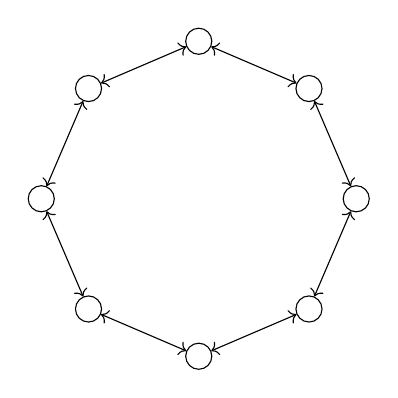
\begin{tikzpicture} [every node/.style={draw,circle}]
            \node (a) at (0, 2)         {};
            \node (b) at (1.4, 1.4)     {};
            \node (c) at (2, 0)         {};
            \node (d) at (1.4, -1.4)    {};
            \node (e) at (0, -2)        {};
            \node (f) at (-1.4, -1.4)   {};
            \node (g) at (-2, 0)        {};
            \node (h) at (-1.4, 1.4)    {};


            \graph[edges={<->}] {
                (a) -- (b) -- (c) -- (d) -- (e) -- (f) -- (g) -- (h) -- (a);
            };
        \end{tikzpicture}
    \end{center}
    \begin{itemize}
        \item We will assume asynchrony, no node or link failures.
    \end{itemize}
\end{frame}


\begin{frame}{Is this possible?}
    \begin{itemize}
        \item True or false? "If processes are identical, no deterministic algorithm can solve leader election in a ring." \pause
        \item True! ...Why? \pause
        \item Proof outline:
        \begin{itemize}
            \item All nodes have same initial state.
            \item If all nodes send the same messages to the left and to the right, all nodes receive the same messages, so no single node can be determined to be \emph{special}.
            \item Proof by induction.
        \end{itemize}\pause
        \item If we assume each node has a unique ID, then the problem is solvable.
    \end{itemize}
\end{frame}


\begin{frame}{Chang-Roberts Algorithm}
    \begin{itemize}
        \item Send IDs clockwise, relay smaller IDs only.
        \item If receiving own ID, output “leader” \& send "terminate".
        \item If receiving “terminate”, relay it \& output “not leader”.
    \end{itemize}
\end{frame}

\begin{frame}{Chang-Roberts Pseudocode}
    \begin{algo}
        \textul{\textsc{ChangRoberts}():}\+
        \\  Send self.ID to clockwise neighbor
        \\  Upon receiving ID from counter-clockwise neighbor\+
        \\      If ID < self.ID:\+
        \\          send ID to clockwise neighbor\-
        \\      If ID == self.ID:\+
        \\          send “terminate” to clockwise neighbor
        \\          output “leader” and terminate\-\-
        \\  Upon receiving “terminate”:\+
        \\      send “terminate” to clockwise neighbor
        \\      output “not leader” and terminate
    \end{algo}
\end{frame}


\begin{frame}{Aside: What does "output" mean?}
    Output to whom?
\end{frame}


\begin{frame}{How do we know this is correct?}
    \begin{itemize}
        \item \emph{Safety}: something bad will never happen.
        \begin{itemize}
            \item \textit{No two nodes output "leader".} That would be bad.
        \end{itemize}
        \item \emph{Liveness}: Something good will happen eventually.
        \begin{itemize}
            \item In an asynchronous model, "eventually" may be a \textit{very} long time. (Aside: why are we okay with this?)
            \item \textit{Every node outputs.}
        \end{itemize}\pause
        \item Fairly straightforward to prove Chang-Roberts satisfies both safety and liveness.
    \end{itemize}
\end{frame}


\begin{frame}{How fast is this? Big-O Analysis.}
    \begin{itemize}
        \item Big-O analysis is used to analyze the \textit{worst-case} runtime of an algorithm without getting bogged down by relatively insignificant details. \pause
        \begin{itemize}
            \item If an algorithm is \emph{$O(n)$}, runtime grows linearly to the size of the input. \pause
            \item For \emph{$O(n!)$} algorithms, runtime grows factorially to the size of the input. \pause
            \item $O(n^2) = O(\frac{n^2}{2}) = O(2000 \cdot n^2 + n\log n + 37) = O(c \cdot n^2)$ \pause
        \end{itemize}
        \item This type of thinking works because computers operate at scale.
    \end{itemize}
\end{frame}

\begin{frame}{}
      \begin{center}
    {\color{sigma@mainblue} \LARGE Questions?}
  \end{center}
\end{frame} 

\begin{frame}{How fast is Chang-Roberts?}
    \begin{itemize}
        \item Time complexity (\# messages between start and finish): \pause $O(n)$
        \begin{itemize}
            \item The smallest ID travels $n$ hops to get back to the leader, then "terminate" travels $n$ hops.\pause
        \end{itemize}
        \item Message complexity (\# messages total): \pause $O(n^2)$
        \begin{itemize}
            \item If every node starts an election at the same time, and IDs are ascending, each of the $n$ IDs travels $n$ hops.
        \end{itemize}
    \end{itemize}
\end{frame}


\begin{frame}{Can we do better?}
    Any ideas?
\end{frame}

\section{Leader Election v2}

\begin{frame}{Hirschberg-Sinclair Algorithm}
    \begin{itemize}
        \item Send IDs in phases with doubling distances.
        \begin{itemize}
            \item In phase $p$, winners of phase $p - 1$ send their ID to both neighbors with a counter set to $2^p$.
            \item Upon receiving an ID, decrement the counter and pass it along.
            \item Upon receiving an ID with counter $= 0$, send an endorsement back.
            \item Upon receiving an endorsement for self, win the round, proceed to next phase.
            \item Upon receiving own ID, output “leader” \& send "terminate".
        \end{itemize}
    \end{itemize}
\end{frame}


\begin{frame}{Hirschberg-Sinclair Correctness}
    \begin{itemize}
        \item Similarly straightforward.\pause
        \item Saftey. \pause Exactly one node can—and will—win every phase. \pause
        \item Liveness. \pause Every process outputs on "terminate".
    \end{itemize}
\end{frame}


\begin{frame}{Hirschberg-Sinclair Efficiency}
    \begin{itemize}
        \item What got better?\pause
        \item Time complexity: $2\cdot (1 + 2 + 4 + 8 + \cdots + n) = O(n)$. \pause
        \item Message complexity:\pause
        \begin{itemize}
            \item In phase $p$, at most $\frac{n}{2^p}$ nodes send their IDs.\pause
            \item In each phase, each node causes at most $4 \cdot 2^{p + 1}$ messages to be sent. \pause
            \item This implies $8n$ messages per phase.
            \item At most $\log n$ phases.
            \item $O(n\log n)$ \quad\quad (\textit{MUCH} better than $O(n^2)$.)
        \end{itemize}
    \end{itemize}
    
\end{frame}



\begin{frame}{Why do we care about using a ring?}
    \begin{itemize}
        \item Flexible; easy to add nodes in the middle of the ring with \emph{consistent hashing}.
        \item We can get tree-like efficiency with \emph{finger tables}:
        \begin{figure}
            \centering
            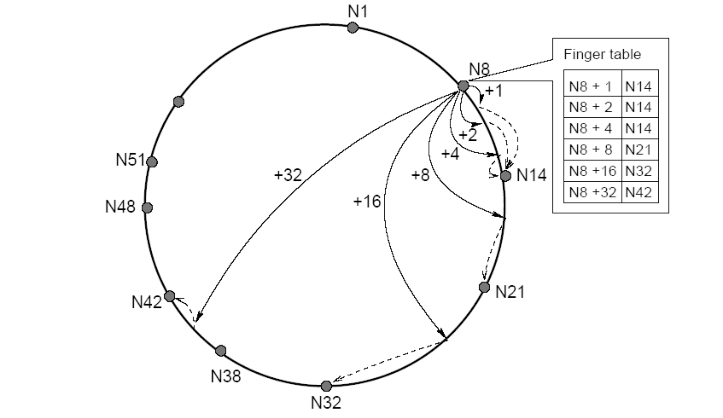
\includegraphics[width=0.5\linewidth]{finger-tables.png}
            \label{fig:placeholder}
        \end{figure}
        \item Why not just use a tree?
    \end{itemize}
\end{frame}


\begin{frame}[allowframebreaks]{Bibliography}
    \tiny
    \begin{itemize}
        \item CS 539 "Distributed Algorithms" lecture slides by Ling Ren (Illinois professor).
        \item My CS 425 "Distributed Systems" notes, based on lecture slides by Indranil Gupta (Illinois professor).
    \end{itemize}
\end{frame}


\end{document}